\chapter{Results}\label{ch:res}

\begin{flushright}{\slshape
    Hofstadter's Law:\\
    It always takes longer than you expect,\\
    even when you take into account Hofstadter's Law.\\ \medskip
    --- Douglas Hofstadter}
\end{flushright}

When designing a system aimed for performance, one has to test the system and
compare it to other solutions to see whether we have gained any mentionable
speedup. As the assignment was to create an array-based image processor, it
would be interesting to see how much more efficient our design is, depending on
the amount of cores the system has.

The first section will go in detail on the performance aspect of the results. We
will here look at throughput, total processing time and other aspects related to
performance, and compare them based on the number of cores we use. In the
following section, we will have a look at the power consumption. We will measure
how much power the system requires running with different cores, and how much
power the system requires to process a single task with different amount of
cores.

{\sc fancy image here}

\section{Performance}

\subsection{SD Card Performance}
\label{sec:performance-sd-card}

As mentioned in Section \ref{sec:avr-spi-issues}, reading data from an
SD card over SPI turned out to be the biggest bottleneck for throughput
in our system. In this section, we will document the optimizations we
made to improve the SD card's read performance.

Table \ref{tab:spi-optimizations-table} shows the gradually improving
performance as we optimized the code. This is also shown in Figure
\ref{fig:spi-optimizations-plot}. Each of the optimizations are
explained in greater detail below.

\begin{description}
	\item[Removed status checking + function inlining] \hfill \\
		The spi\_send function busy-waited on the TXEMPTY flag for each
		byte it transmitted. In our case of alternating sends and reads,
		we do not have to check whether the SPI send register is empty
		every time. Inlining spi\_read and spi\_write also helped,
		although -O1, -O2 or -O3 would have done this for us.
	\item[Less SPI status register polling] \hfill \\
		In spi\_read, two conditions are busy-waited on before
		returning: whether the send register is empty, and whether the
		receive buffer is full yet. We only have to check the latter of
		these conditions.
	\item[Increased clock rate] \hfill \\
		Our CPU and main bus is driven by an external 12MHz crystal
		oscillator and the SPI clock frequency is calculated by dividing
		this by an integer number. We kept this divisor to be either 1
		or 2 (so SPI ran at either the same or half the speed of the
		CPU). Increasing to clock rate from 12MHz to 78 MHz boosted the
		speed from 157kB/s to 456 kB/s.
	\item[Compiler optimizations] \hfill \\
		Turning on compiler optimizations improved increase performance
		by another 14\%. There was no noticeable difference in
		performance from -O1, -O2 or -O3. However, compiler
		optimizations had a more profound effect on the overall system
		performance. We did not benchmark this extensively, but it was
		probably caused by optimizations the compiler made to the \ac{LENA}
		communication code.
	\item[Bypass FAT and use multiple block reads] \hfill \\
		We patched the framework code to support multiple block reads.
		Apparently, this was not something the FAT driver was able to
		take full advantage of out of the box. It was easier to simply
		bypass the file system than to try to fix it, so that is what we
		did.
		
		By reading the blocks directly from the SD card, we could read
		all 150 blocks of a picture in one function call. Limiting the
		file system to the first half of the SD card and add metadata
		files containing the block offsets into the second half of the
		card was easy. This more than doubled our performance, from 515
		kB/s to 1172 kB/s.
\end{description}

\TODO{This must be rewritten}
After implementing these optimizations, the \ac{SCU} was capable of pushing out around
12 FPS to the \ac{LENA}, around 920 kB/s. As we managed to reach our goal of 10
FPS, we did not optimize it any further. However, using the \ac{PDCA}, we could
have effectively eliminated the 25\% time spent sending to the \ac{LENA} while
the \ac{SD} card waited. Thus, giving as a frame rate of around 16
FPS. 
\begin{table}[H]
  \centering
  \begin{tabularx}{\textwidth}{c X r} \toprule
    \thx{Milestone} & \thx{Description} & \thx{Performance} \\
    \midrule
    1 & Baseline before optimization & 74.87 kB/s \\
    2 & Less status checking in {\tt spi\_send} plus inlining & 137.00 kB/s \\
    3 & Less \ac{SPI} status register polling & 156.59 kB/s \\
    4 & Clock rate of 20MHz, 10MHz \ac{SPI} & 214.40 kB/s \\
    5 & Clock rate of 20MHz, 20MHz \ac{SPI} & 243.00 kB/s \\
    6 & Clock rate of 40MHz, 20MHz \ac{SPI} & 327.80 kB/s \\
    7 & Clock rate of 48MHz, 24MHz \ac{SPI} & 369.50 kB/s \\
    8 & Clock rate of 60MHz, 30MHz \ac{SPI} & 423.40 kB/s \\
    9 & Clock rate of 72MHz, 36MHz \ac{SPI} & 432.70 kB/s \\
    10 & Clock rate of 78MHz, 39MHz \ac{SPI} & 455.80 kB/s \\
    11 & Turn on {\tt -O1} & 521.70 kB/s \\
    12 & Turn on {\tt -O2} & 523.40 kB/s \\
    13 & Turn on {\tt -O3} & 515.30 kB/s \\
    14 & Bypass \ac{FAT} and use multiple block reads & 1171.90 kB/s \\ 
    \bottomrule
  \end{tabularx}
  \caption[SPI Read Performance]{The read performance over \ac{SPI} at various
    milestones.}
  \label{tab:spi-optimizations-table}
\end{table}

\begin{figure}[H]
  \centering
  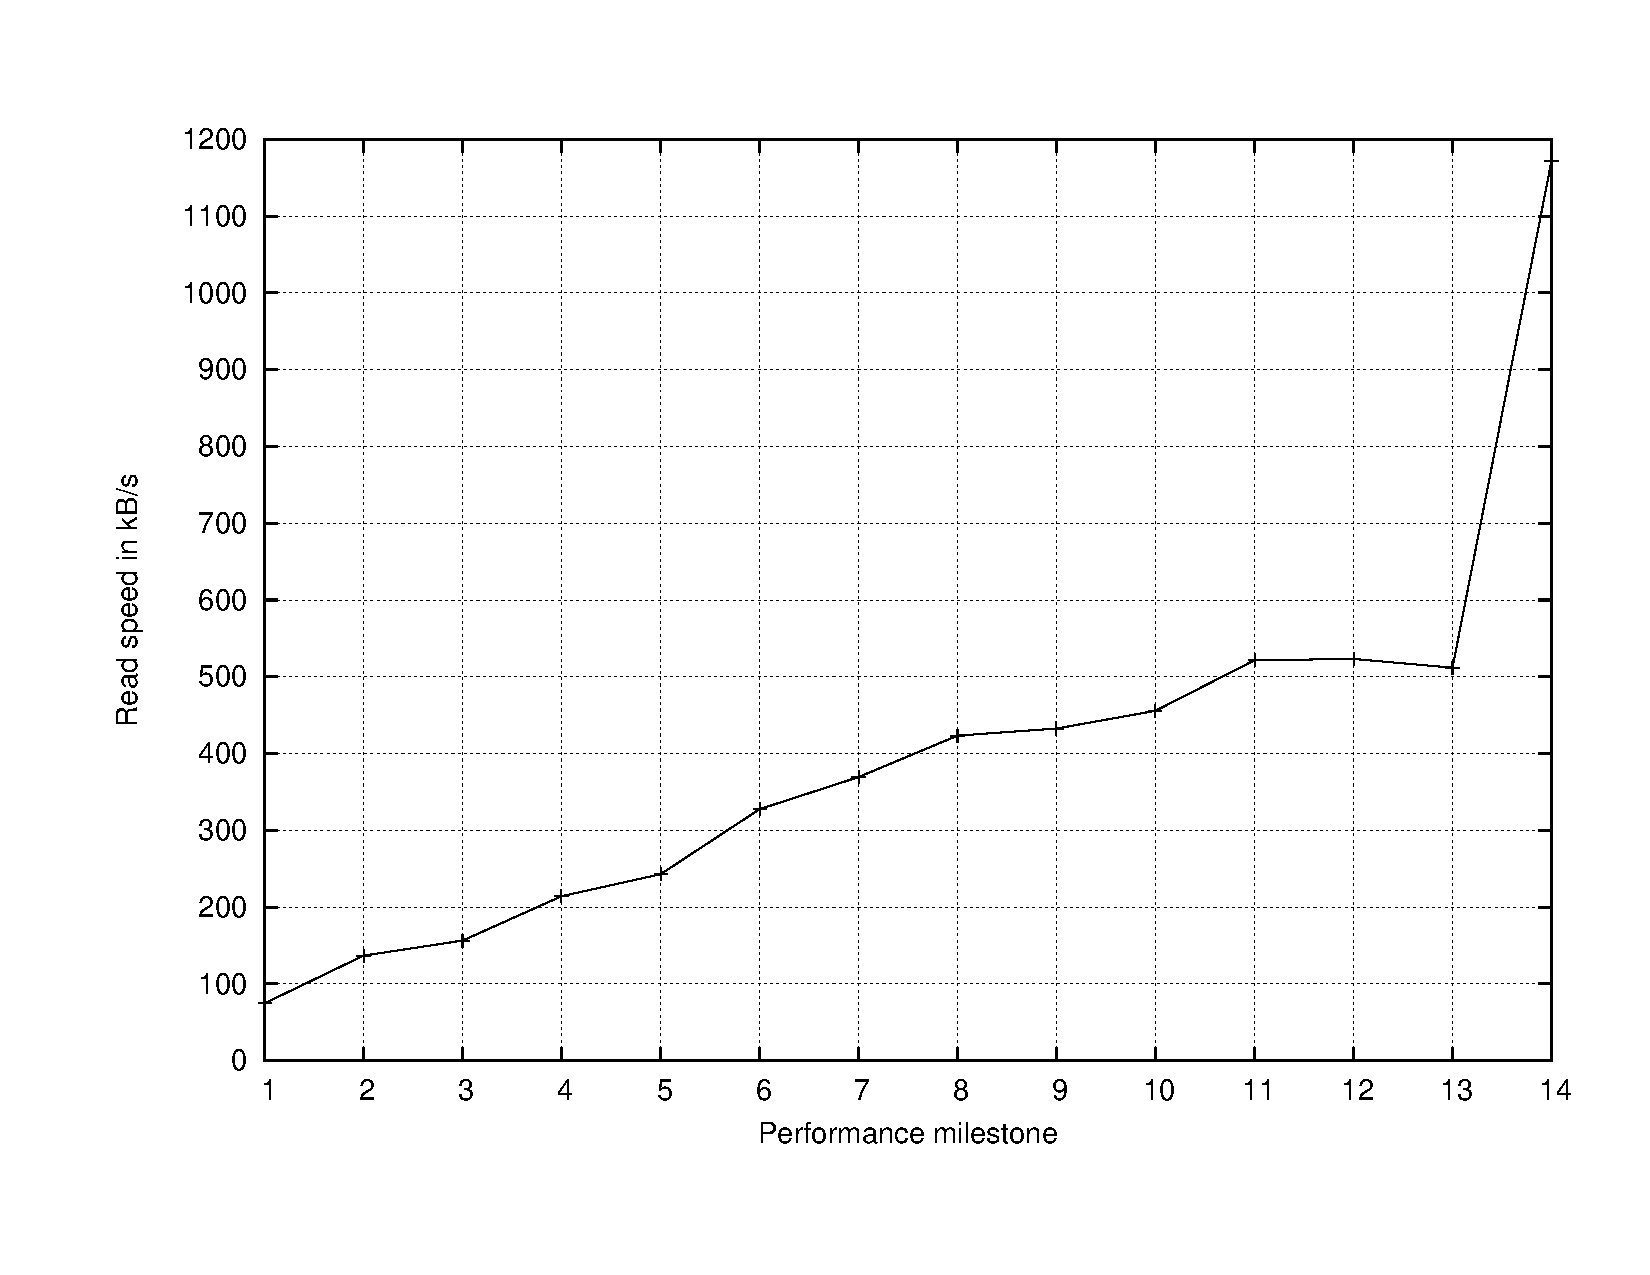
\includegraphics[width=\textwidth]{fig/avr/spi-optimizations-plot.pdf}
  \caption[SPI Optimizations Plot]{The results from Table
    \ref{tab:spi-optimizations-table} plotted. Milestones are along the
    $x$-axis and read performance along the $y$-axis.}
  \label{fig:spi-optimizations-plot}
\end{figure}


\subsection{LENA}
\TODO{Her skriver vi litt om figuren og tabellen nedenfor...}

\begin{table}[h!]
\centering
\begin{tabular}{c|r|rrr|r} \toprule
	\multirow{2}{*}{\textbf{Program}} &
        \multirow{2}{*}{\textbf{Frame rate}} &
        \multicolumn{3}{c|}{\textbf{Current through power planes}} &
        \multirow{2}{*}{\textbf{Power}} \\
        & &
        \textbf{3.3 V} &
        \textbf{2.5 V} &
        \textbf{1.2 V} & \\
	\midrule
	\emph{Idle} & - & 347 mA & 44 mA & 77 mA & 5.6 W \\
	1 & 21 fps & 375 mA & 37 mA & 69 mA & 5.8 W \\
        2 & 18 fps & 375 mA & 37 mA & 71 mA & 5.8 W \\
        3 & 13 fps & 370 mA & 37 mA & 65 mA & 5.7 W \\
        4 & 13 fps & 375 mA & 37 mA & 67 mA & 5.7 W \\
        5 & 13 fps & 363 mA & 37 mA & 75 mA & 5.7 W \\ \bottomrule
\end{tabular}
\caption[LENA results]{LENA performance and power results.}
\label{tab:lena-benchmark-table}
\end{table}

\begin{figure}[h!]
\centering
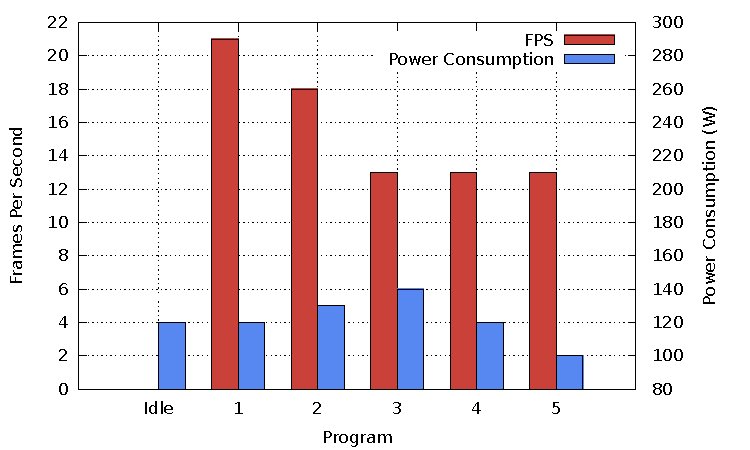
\includegraphics[width=\textwidth]{fig/res/lena-benchmark-plot.pdf}
\caption[LENA results]{The LENA results from Table
\ref{tab:lena-benchmark-table}.}
\label{fig:lena-benchmark-plot}
\end{figure}


\section{Power}

In this section, there will be data as specified in the disposition. We will run
a program which requires data from neighbours, and see how much power the
different programs take based on the amount of cores. We will then explain
eventual results. Compared to the other group, we have completely ignored power
consumption, and e.g. our voltage regulators (?) just burn off the additional
power they get, so it's likely a drastic difference here.

There will also be some fancy plots and tables here to show the (incredibly
high) power consumption.

